\chapter{Reisebranche}
\label{chap:Reisebranche}
Die Reisebranche wird von wenigen Anbietern auf dem Markt bedient, was zu einem sogenannten Oligopol führt. Betrachtet man den größten Reiseportalbetreiber in Deutschland aus dem Jahr 2017, Booking.com, so fällt auf, dass er hierzulande mit weitem Abstand die Liste der umsatzstärksten Unternehmen in diesem Bereich anführt \cite[vgl.][]{FVW2017}. Das ist nicht verwunderlich, vereint die Booking Holding unter sich auch Marken wie Agoda, Momondo oder Kayak \cite[vgl.][]{Booking2019}. Beim zweitgrößten Betreiber Expedia verhält es sich ähnlich; auch hier gibt es Tochterfirmen wie Trivago, Homeaway und Ebookers \cite[vgl.][]{Expedia2019}.\\
Aufgrund des geringen Marktdrucks der Anbieter werden häufig veraltete IT-Systeme eingesetzt, welche zu Sicherheitslücken neigen. Im Jahr 2017 kam es so beispielsweise zu Hackerangriffen auf das Computerreservierungssystem von Sabre, einer der Top drei Firmen auf diesem Gebiet \cite[vgl.][]{Mathews2017}.

Um das Missverhältnis zwischen Angebot und Nachfrage auszugleichen sowie eine Erneuerung der IT anzustreben, engagieren sich Firmen wie Winding Tree, um mittels Blockchain und Smart Contracts eine direkte Verbindung zwischen Airlines bzw. Hotels und den Buchenden herzustellen (siehe Abbildung \ref{fig:windingTreeOverview}). Um die Notwendigkeit dazu zu untermauern hebt Winding Tree in ihrem Whitepaper als Ausgangspunkt vor allem die hohen Gebühren hervor, die die klassischen Intermediäre bei erfolgreicher Vermittlung berechnen \cite[vgl.][S. 2 f.]{WT2019}.

\begin{figure}[h!]
  \centering
  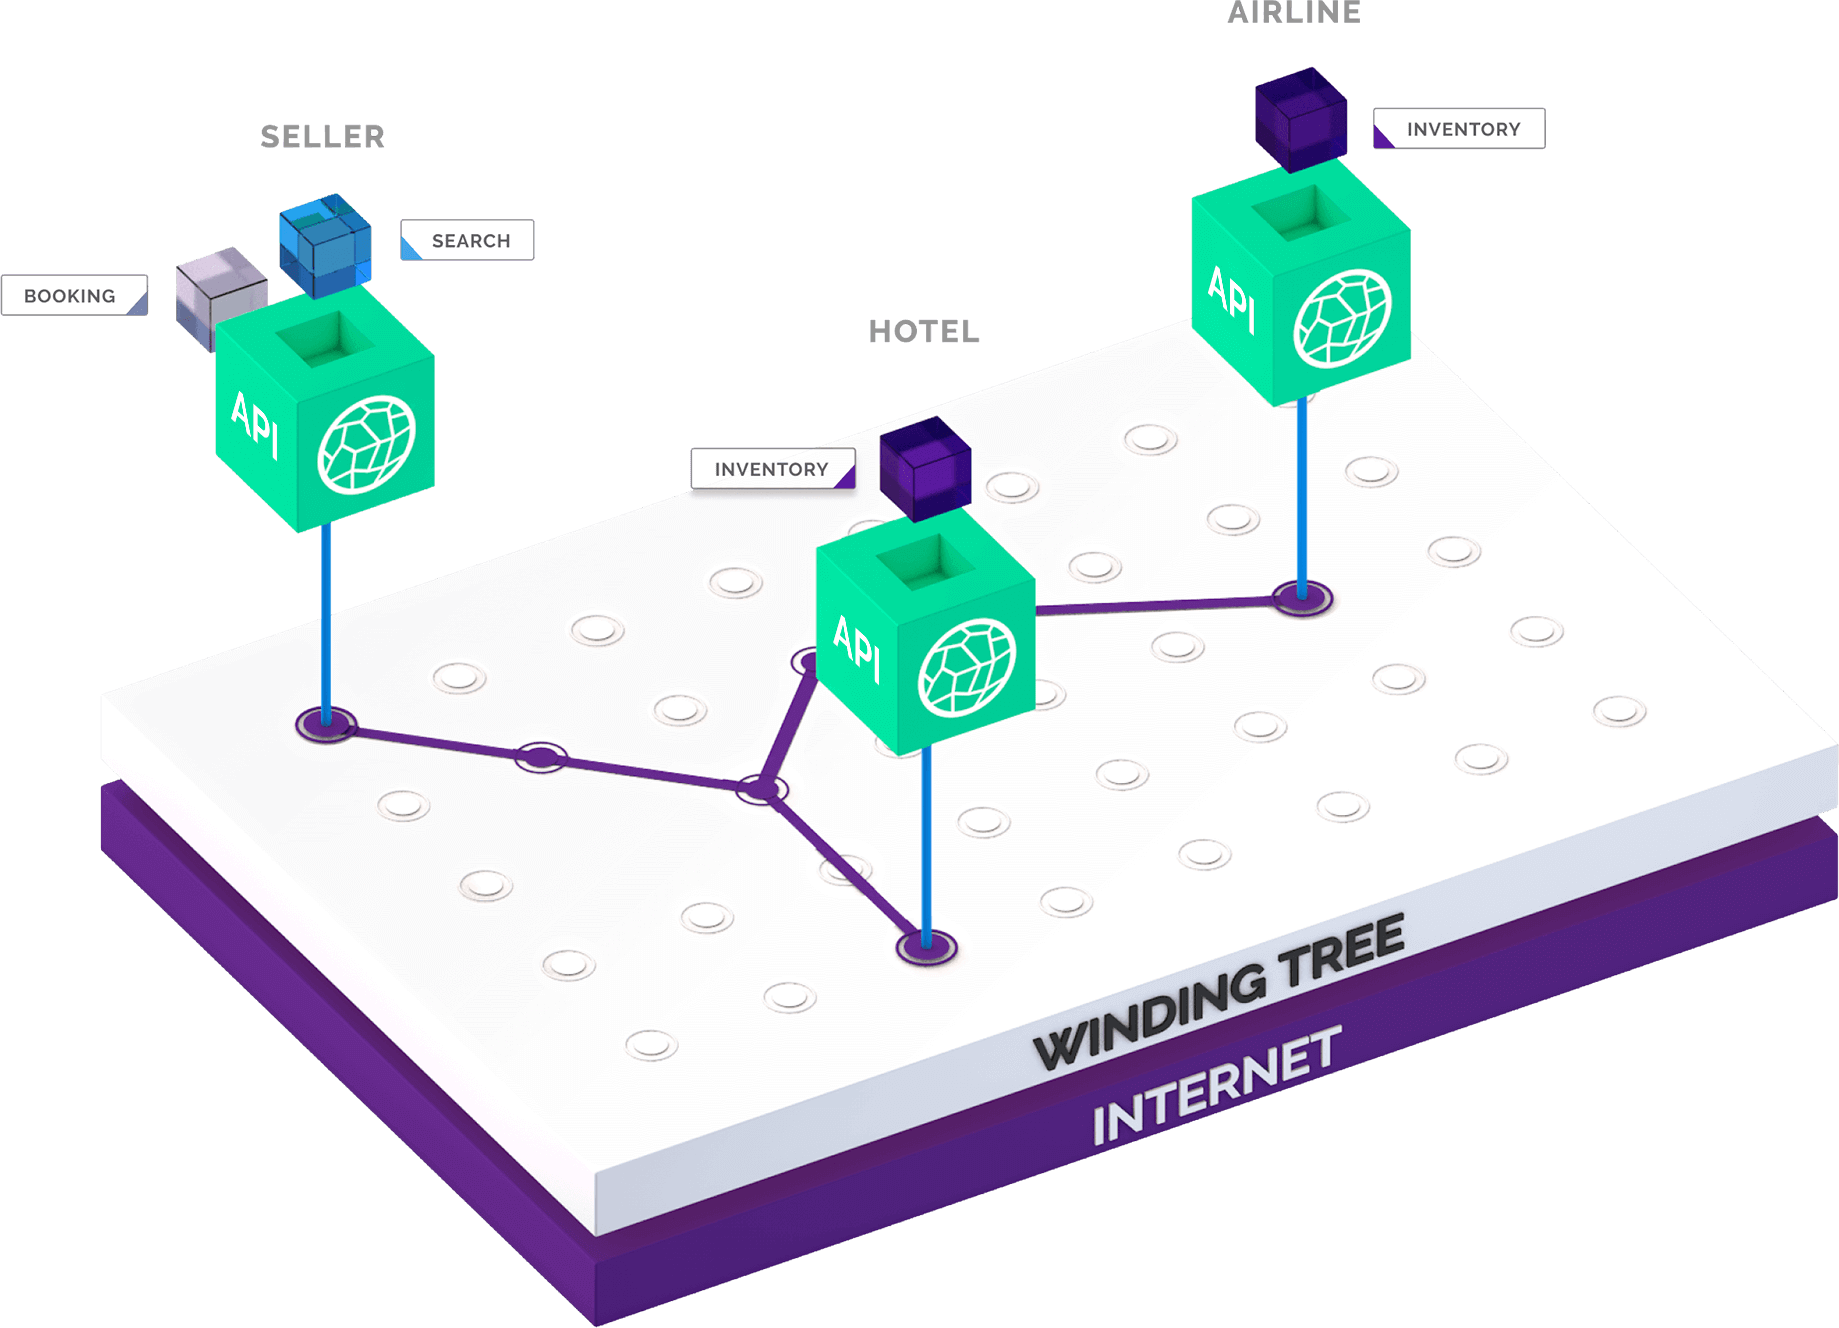
\includegraphics[width=\textwidth]{Bilder/WindingTreeOverview.png}
  \caption[Winding Tree Überblick]{Winding Tree Überblick \cite{WTWebsite2019}}
  \label{fig:windingTreeOverview}
\end{figure}

Winding Tree bietet lediglich die Plattform inklusive Schnittstellen zur Abwicklung der Geschäftsbeziehungen an, alle weiteren Anwendungen (z. B. Benutzeroberflächen) müssen von den Teilnehmern selbst implementiert werden. Dabei stehen als Hilfestellung allerdings auch Referenzimplementierungen in JavaScript unter der Apache-2.0-Lizenz auf Winding Trees GitHub Account bereit \cite{WTGitHub2019}.\\
Dass dies nicht nur eine Nischenlösung ist, wird beim Blick auf die Industriepartner bewusst: Neben Hotelketten wie Nordic Hotels sind vor allem große europäische Airlines auf der Plattform vertreten. Dazu gehören unter anderem auch AirFrance, KLM, SWISS, Eurowings und die Lufthansa \cite{WTWebsite2019}.

- Líf-Token -> Notwendigkeit, Grundlage, ganz kurz Token Event; Market Validation Mechanism interessanter [Seite 2 und 3 halb]\\
- Ablauf allgemein (Beispiel aus Whitepaper) + Contracts genauer (siehe GitHub) [Seite 3 halb und 4]\\#
- Kritik am System [Seite 4] \\